\subsection*{Problema 11}

\noindent\textbf{Enunciado:} \\
Calcular la integral indefinida:
\begin{align*}
\int \frac{x^4}{x^4 + 2x^2 + 1} \, dx
\end{align*}

\noindent\textbf{Solución:} \\
Primero, notemos que el denominador es un trinomio cuadrado perfecto. Podemos reescribirlo como:
\begin{align*}
x^4 + 2x^2 + 1 = (x^2 + 1)^2
\end{align*}

Sustituyendo esto en la integral, la expresión se convierte en:
\begin{align*}
\int \frac{x^4}{(x^2 + 1)^2} \, dx
\end{align*}

Siguiendo la sugerencia de expresar el numerador de forma conveniente, reescribimos $x^4$ como:
\begin{align*}
x^4 &= (x^2 + 1)^2 - 2(x^2 + 1) + 1
\end{align*}

Sustituyendo este resultado en el integrando, dividimos término a término:
\begin{align*}
\frac{x^4}{(x^2+1)^2} &= \frac{(x^2+1)^2}{(x^2+1)^2} \\
&\quad - \frac{2(x^2+1)}{(x^2+1)^2} + \frac{1}{(x^2+1)^2}
\end{align*}

Simplificando cada término algebraicamente, obtenemos:
\begin{align*}
&= 1 - \frac{2}{x^2+1} + \frac{1}{(x^2+1)^2}
\end{align*}

Ahora, integramos cada parte por separado:
\begin{align*}
\int 1 \, dx &= x \\
\int \frac{-2}{x^2+1} \, dx &= -2 \arctan(x)
\end{align*}

Para la última integral, $\int \frac{1}{(x^2+1)^2} \, dx$, utilizamos la sustitución trigonométrica $x = \tan(\theta)$, de donde $dx = \sec^2(\theta) \, d\theta$:
\begin{align*}
\int \frac{\sec^2(\theta)}{(\tan^2(\theta)+1)^2} \, d\theta &= \int \frac{\sec^2(\theta)}{(\sec^2(\theta))^2} \, d\theta \\
&= \int \frac{1}{\sec^2(\theta)} \, d\theta \\
&= \int \cos^2(\theta) \, d\theta
\end{align*}

Usando la identidad del ángulo doble:
\begin{align*}
\int \frac{1 + \cos(2\theta)}{2} \, d\theta &= \frac{\theta}{2} + \frac{\sin(2\theta)}{4} \\
&= \frac{\theta}{2} + \frac{\sin(\theta)\cos(\theta)}{2}
\end{align*}

Volviendo a la variable original $x$:
\begin{align*}
&= \frac{\arctan(x)}{2} + \frac{x}{2(x^2+1)}
\end{align*}

Sumando todas las partes y agregando la constante de integración $C$, obtenemos la solución final:
\begin{align*}
\int \frac{x^4}{x^4 + 2x^2 + 1} \, dx &= x - 2\arctan(x) \\
&\quad + \frac{\arctan(x)}{2} \\
&\quad + \frac{x}{2(x^2+1)} + C
\end{align*}

Agrupando los términos semejantes de $\arctan(x)$:
\begin{align*}
&= x - \frac{3}{2}\arctan(x) \\
&\quad + \frac{x}{2(x^2+1)} + C
\end{align*}

\begin{figure}[H]
	\centering
	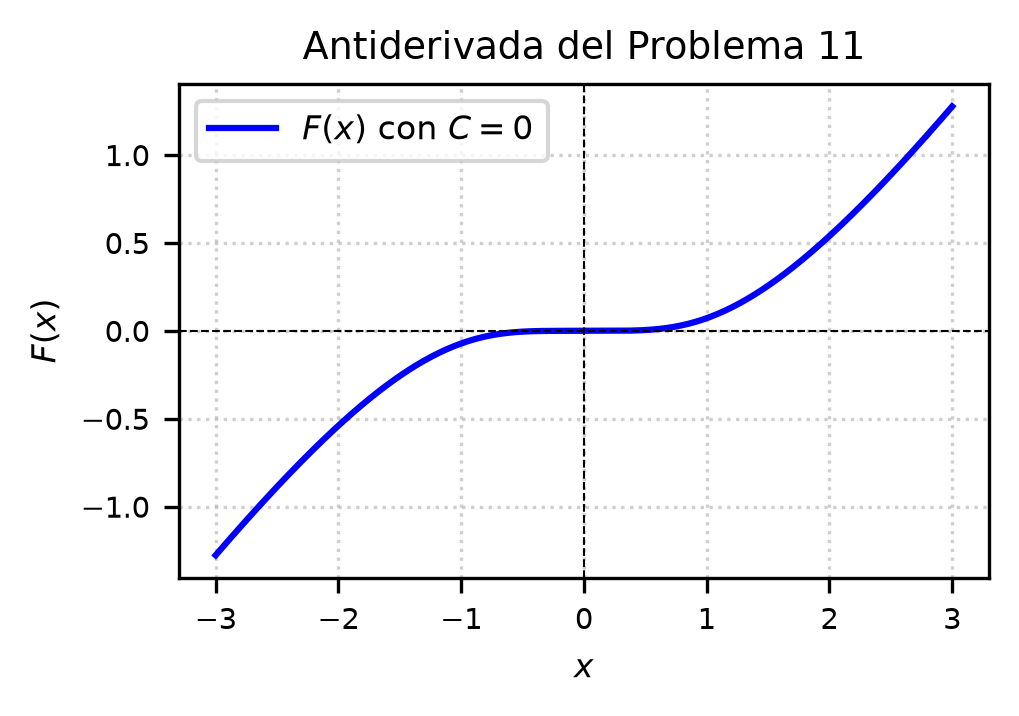
\includegraphics[width=\columnwidth]{semana_03/graficas/SEM03_P11_grafica.png}
	\caption{Representación gráfica de $f(x)$ y su antiderivada $F(x)$ evaluada para la constante de integración $C = 0$ (Problema 11).}
	\label{fig:problema11}
\end{figure}
